\section{Three-flavor Oscillation Measurement}
\label{sec:three-flavor-measurement}
The first measurement that is run using the data sample described in this work is the measurement of the atmospheric mixing angle $\theta_{23}$ and the mass splitting $\Delta m^2_{32}$. The experimental setup of DeepCore is ideally suited for this measurement, because the first valley of maximum disappearance for muon neutrinos passing through the entire diameter of the Earth is expected to lie between 20~GeV and 30~GeV as shown in \reffig{three-flavor-oscprob}. The parameter $\Delta m^2_{32}$ changes the position of the oscillation valley, while $\theta_{23}$ changes its depth. In the analysis histogram, this disappearance effect is apparent even by eye alone in the PID channel for highly track-like events as shown in \reffig{nominal-hist-null-hypo}. For this measurement, oscillation probabilities are calculated in the three-flavor oscillation scheme including matter effects. The matter profile of Earth is modeled as a shells of constant density following the Preliminary Reference Earth Model (PREM)\sidecite{PREM}. The Monte-Carlo simulated events are weighted in a staged procedure where each stage updates the event weights according to flux, cross-sections and oscillation probabilities\sidecite{PISA}. The oscillation probabilities are calculated using a \textsc{Python} implementation of the Barger~et~al.\sidecite{barger-oscillations} calculation.

\begin{figure}
    \centering
    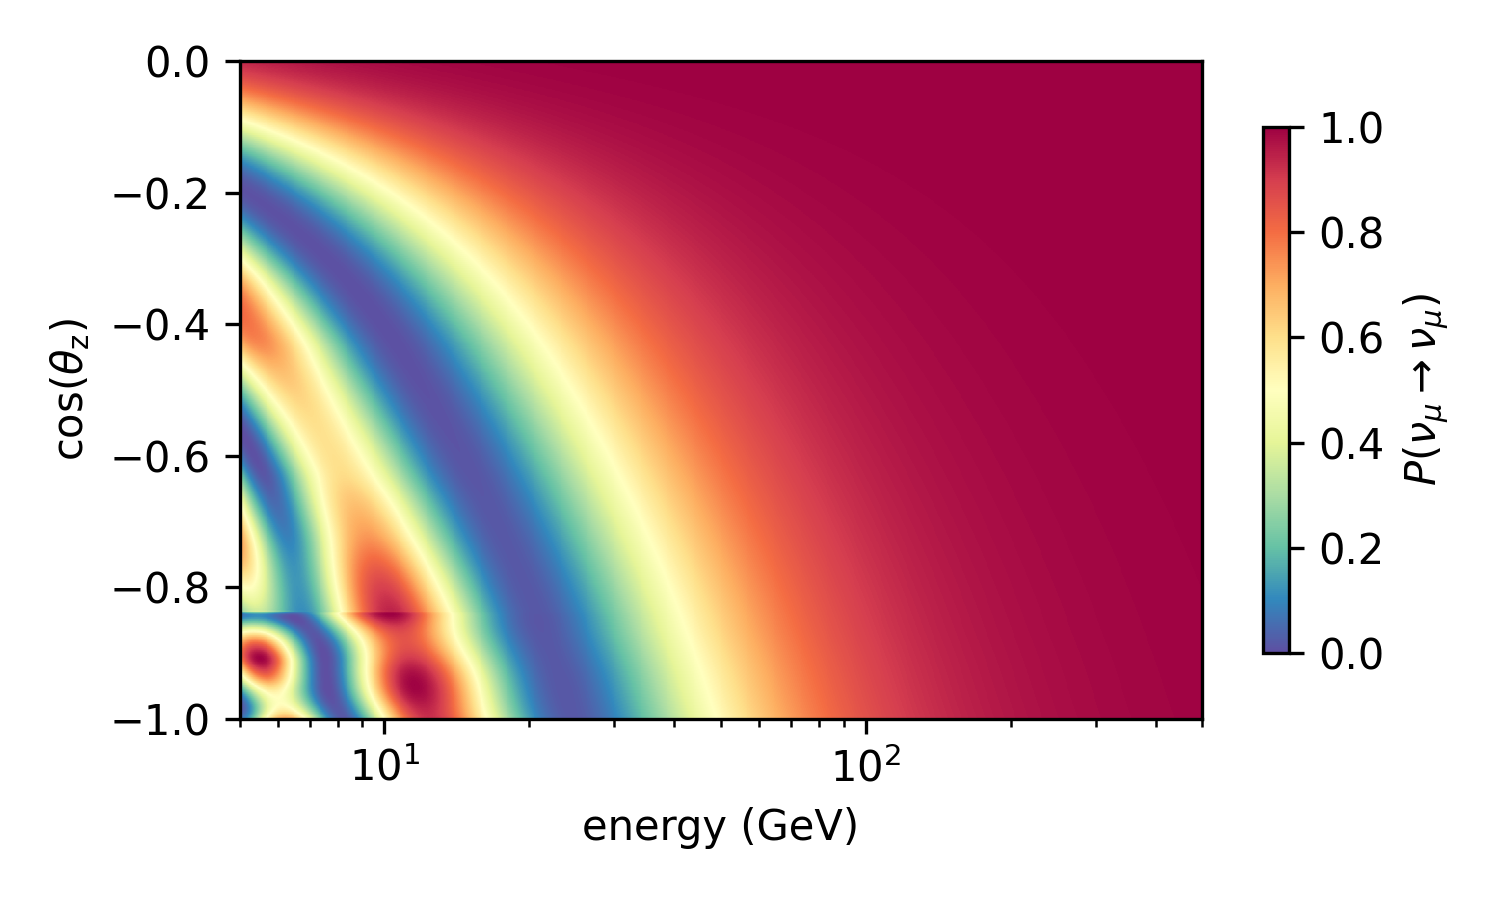
\includegraphics[width=0.9\linewidth]{figures/measurement/three_flavor/numu_surv_prob_no_sterile_no_text.png}
    \caption{Muon-neutrino survival \todo[inline]{find parameters} probability calculated using}
    \label{fig:three-flavor-oscprob}
\end{figure}

\subsection{Selection of Free Parameters}
\label{sec:std-osc-free-parameters}

When including all plausible sources of systematic uncertainties that are described in \refsec{systematic-uncertainties}, the test statistic from \refeq{mod-chi2} would have to be optimized with respect to 28 nuisance parameters: Five describing the uncertainty of the detector (\refsec{detector-unc}), 18 parameters describing the uncertainties on the hadronic interaction model (\refsec{barr-scheme}) and cosmic ray spectrum, four parameters for uncertainties on the neutrino cross-sections (\refsec{xsec_systs}), and the scale of the muon background (\refsec{atm-muons-systematic}). Together with the two physics parameters, this would require an optimization in 30 dimensions to run the analysis. To reduce this computational burden, the potential bias and its significance that could plausibly be produced by each parameter is assessed, and the value of parameters that are found to have a negligible impact is fixed to its global best-fit value. The impact of each parameter is tested as follows: First, pseudo-data \emph{without} statistical fluctuations is produced from simulation where the value of the parameter to be tested is increased by $1\sigma$ if it has a Gaussian prior, or half-way to its upper boundary if it does not have a prior. The histograms are then fit back while keeping the parameter to be tested fixed at its nominal value. This fit is done once with the physics parameters ($\theta_{23}$ and $\Delta m^2_{31}$) fixed at the value that was used to create the pseudo-data, and once with the physics parameters left free. The difference in the test statistic $\chi^2_{\mathrm{mod}}$ between the free fit and the fit with physics parameters fixed to the truth, $\Delta \chi^2_{\mathrm{mod}}$, is referred to as \emph{mis-modeling}. The p-value of the mis-modeling, calculated under the assumption that it should follow a $\chi^2$-distribution with two degrees of freedom, can be interpreted as the significance with which the analysis would have rejected the true physics value \emph{solely} due to the exclusion of the parameter in question. This test neglects any global offset to the test statistic, since it would not affect the estimate of the confidence limits for the physics parameters.
\begin{figure}
    \centering
    \missingfigure[figwidth=0.8\linewidth,figheight=0.7\linewidth]{Mis-modeling grid produced for one parameter in the mis-modeling ranking test.}
    \caption{Grid of $\Delta \chi^2_{\mathrm{mod}}$ values showing the impact of one parameter being pulled by $1\sigma$.}
    \label{fig:systematic-impact-mismod-example}
\end{figure}
The test described above is repeated for a grid of true values of $\theta_{23}$ and $\Delta m^2_{31}$ spanning the entire range of values that is not strongly excluded by other measurements, producing one value for $\Delta \chi^2_{\mathrm{mod}}$ at each grid point as shown in \reffig{systematic-impact-mismod-example}. The largest value of $\Delta \chi^2_{\mathrm{mod}}$ from the entire grid produced for one parameter represents the \emph{maximum mis-modeling} for that parameter. Taking the maximum mis-modeling for all parameters, one can produce a ranking of the impacts of all parameters of the analysis as shown in \reffig{systematic-impact-mismod-ranking}. Parameters for which the maximum mis-modeling lies below a conservatively chosen value of $\Delta \chi^2_{\mathrm{mod}} < 0.01$ are fixed to their global best-fit value in the analysis, reducing the total number of free parameters to XX\todo{get the exact number of parameters}. The complete list of all parameters of the analysis, their priors and their allowed ranges can be found in \reftab{sys-params-three-flavor} in the appendix.
\begin{figure}
    \centering
    \missingfigure[figwidth=0.6\linewidth, figheight=0.8\linewidth]{Mis-modeling ranking for the three-flavor analysis.}
    \caption{Ranking of $\Delta \chi^2_{\mathrm{mod}}$ values for all nuisance parameters considered for the three-flavor oscillation analysis.}
    \label{fig:systematic-impact-mismod-ranking}
\end{figure}

\subsection{Analysis Checks}
Before running the analysis on real data, its robustness is assessed on pseudo-data produced with MC simulated data sets. Once the robustness on pseudo-data has been established, the analysis is first run \emph{blindly}, that is, without showing the analyzer the results of the physics parameters and only revealing a set of goodness-of-fit variables that has been chosen in advance. Only when the values of these variables lie within the plausible range that can be expected from purely statistical fluctuations are the actual fit values of the measured parameters revealed. 

\subsubsection{Robustness of the minimization}
\label{sec:three-flavor-inject-recover-test}
The free fit of the physics parameters $\theta_{23}$ and $\Delta m^2_{31}$ is run separately once for the lower octant ($\theta_{23} < 45^\circ$) and once for the upper octant ($\theta_{23} > 45^\circ$) to break the degeneracy between the octants. Each fit uses the \textsc{scipy}\cite{2020SciPy-NMeth} implementation of the \textsc{L-BFGS-B} algorithm\cite{l-bfgs-b} to find the parameter values that minimize the $\chi^2_{\mathrm{mod}}$ test statistic. To ensure that the minimization will always converge to the global optimum for any true value of the physics parameters, pseudo-data without statistical fluctuations (also referred to as an \emph{Asimov} test set) is produced on a grid spanning all values that are not strongly excluded by other experiments and a fit is run for each grid point. Since there are no statistical fluctuations, the fit is expected to always converge exactly to the injected true value. As can be seen in the result shown in \reffig{three-flavor-asimov}, the convergence of the minimizer is robust everywhere. 
\begin{figure}
    \centering
    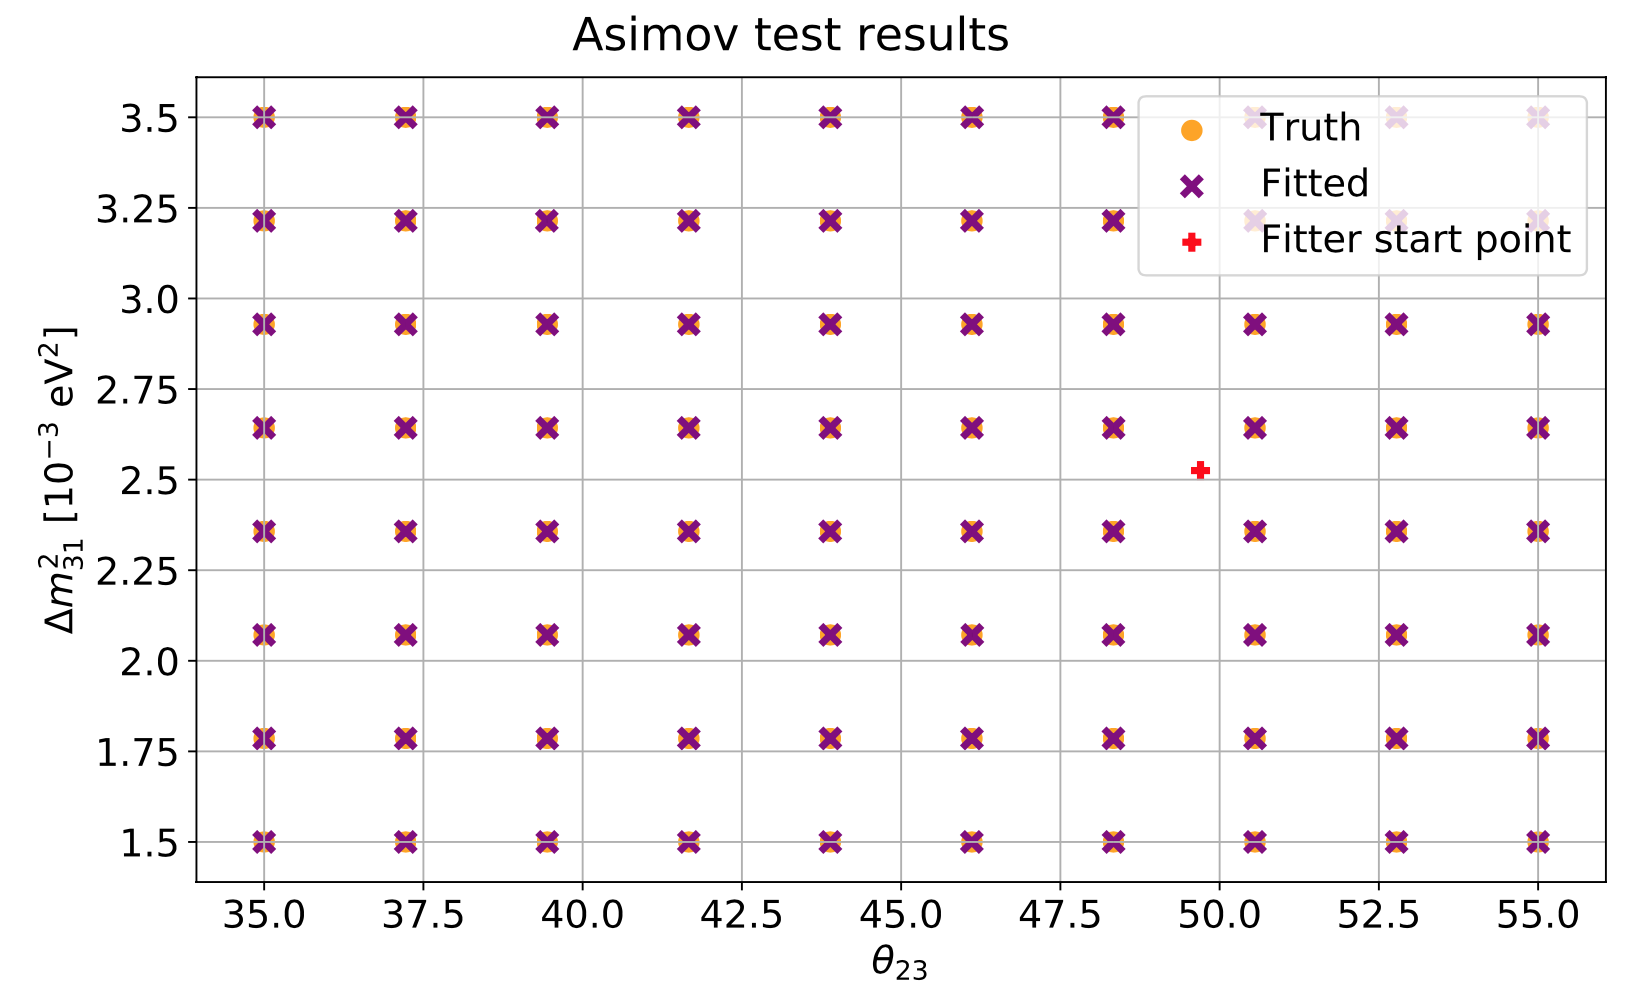
\includegraphics[width=0.9\linewidth]{figures/measurement/three_flavor/asimov_test/inject_recover_map.png}
    \caption{Asimov inject/recover test result for the three-flavor oscillation analysis.}
    \label{fig:three-flavor-asimov}
\end{figure}

\subsubsection{Ensemble tests}
\label{sec:three-flavor-ensemble}
To get expected distributions of the test statistic and parameter fluctuations, the analysis is run on an ensemble of fluctuated pseudo-data. For every trial of the ensemble, the expectation value in every analysis bin is first drawn from a normal distribution centered at the MC expectation with a standard deviation corresponding to the MC uncertainty. Using these sampled expectation values, the bin-count is drawn from a Poisson distribution independently in every bin. This sampling scheme ensures that the fluctuations reflect both the MC uncertainty and the Poisson fluctuations expected in data. A free fit is run on every trial, producing a set of best fit parameters, one value for the total $\Delta \chi^2_{\mathrm{mod}}$ test statistic as well as the contribution of every bin in the analysis histogram to this total value. The distribution for the fit parameters and their pull from their injected values from the ensemble is shown in \reffig{three-flavor-ensemble-param}. The distributions for all parameters are centered on the injected value, demonstrating that the fit is behaving robustly under the expected fluctuations. 

\begin{figure} 
    \centering
    \begin{subfigure}[t]{0.99\textwidth}
        \centering
        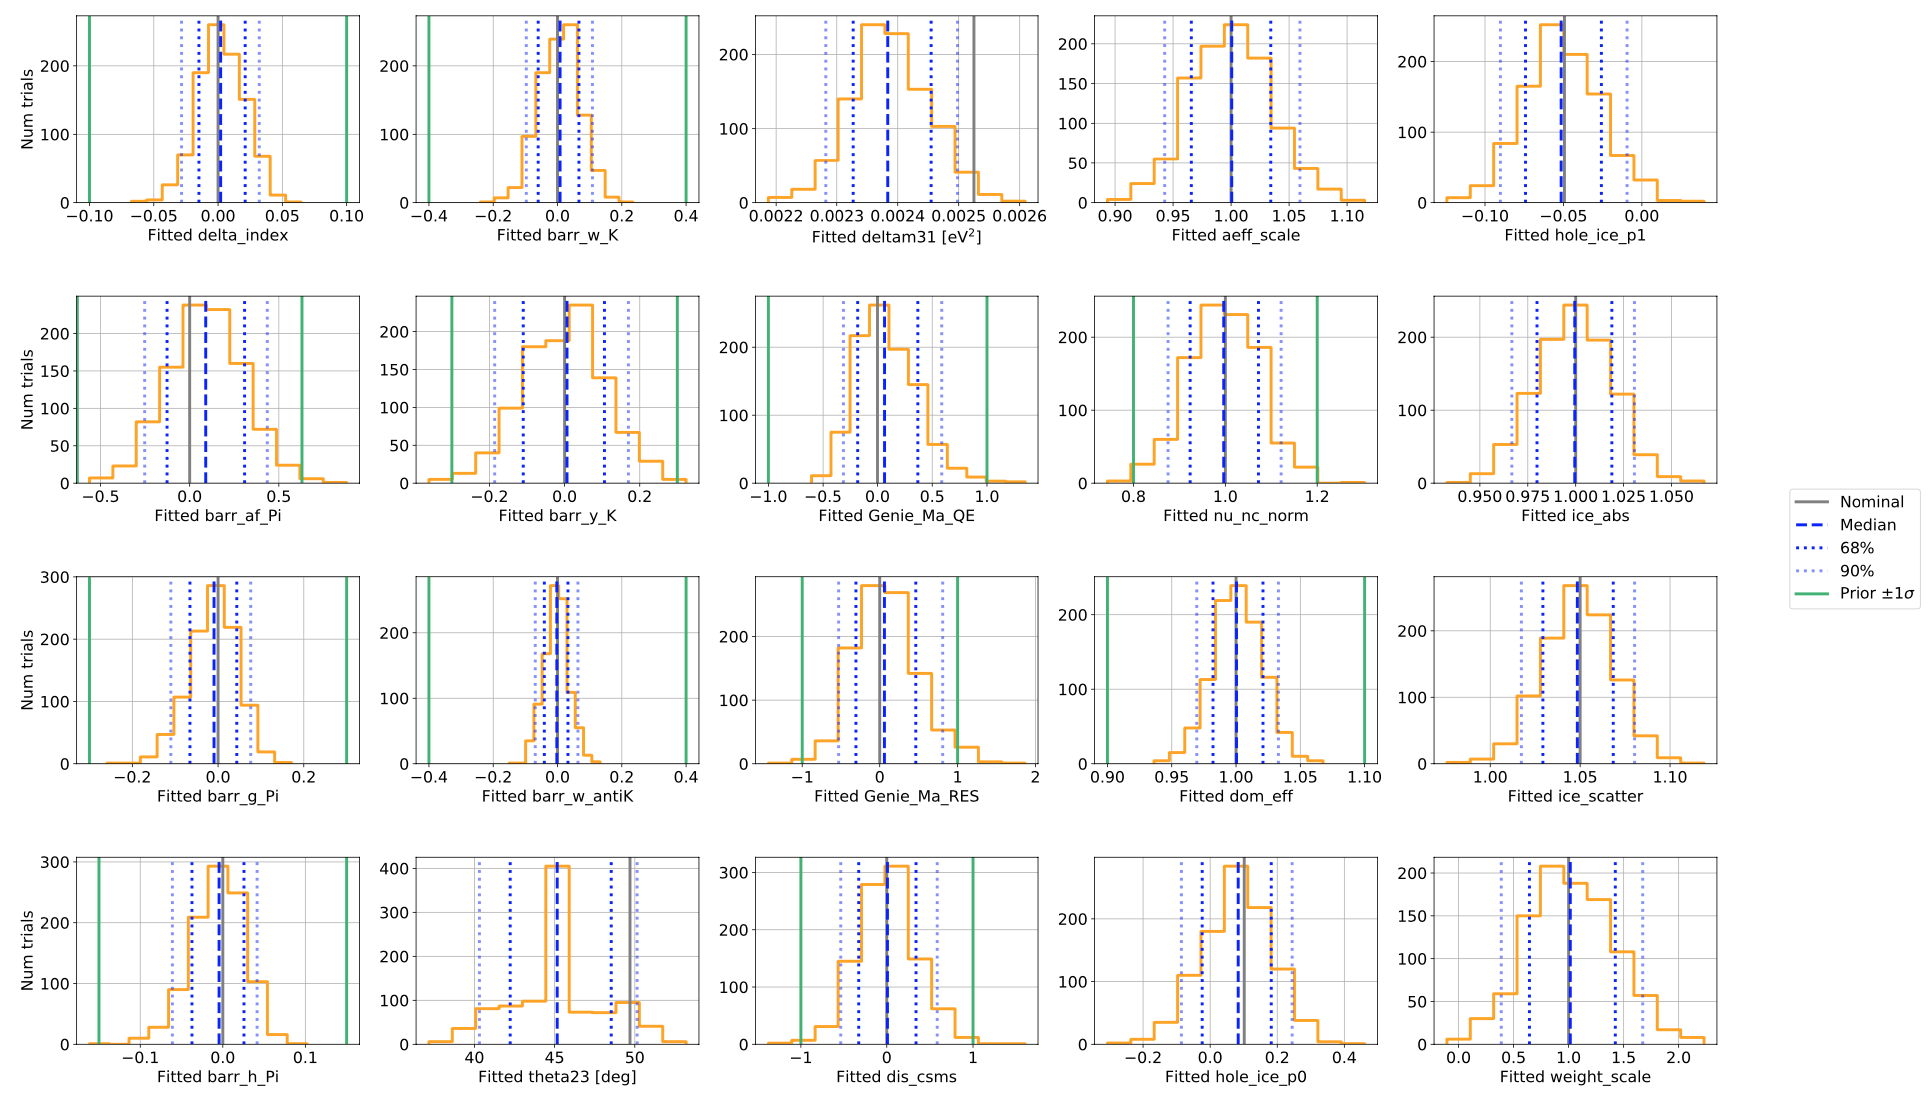
\includegraphics[width=0.99\textwidth]{figures/measurement/three_flavor/ensemble_pre_fit/ensemble_fitdist.png}
    \end{subfigure}
    \begin{subfigure}[t]{0.65\textwidth}
        \centering
        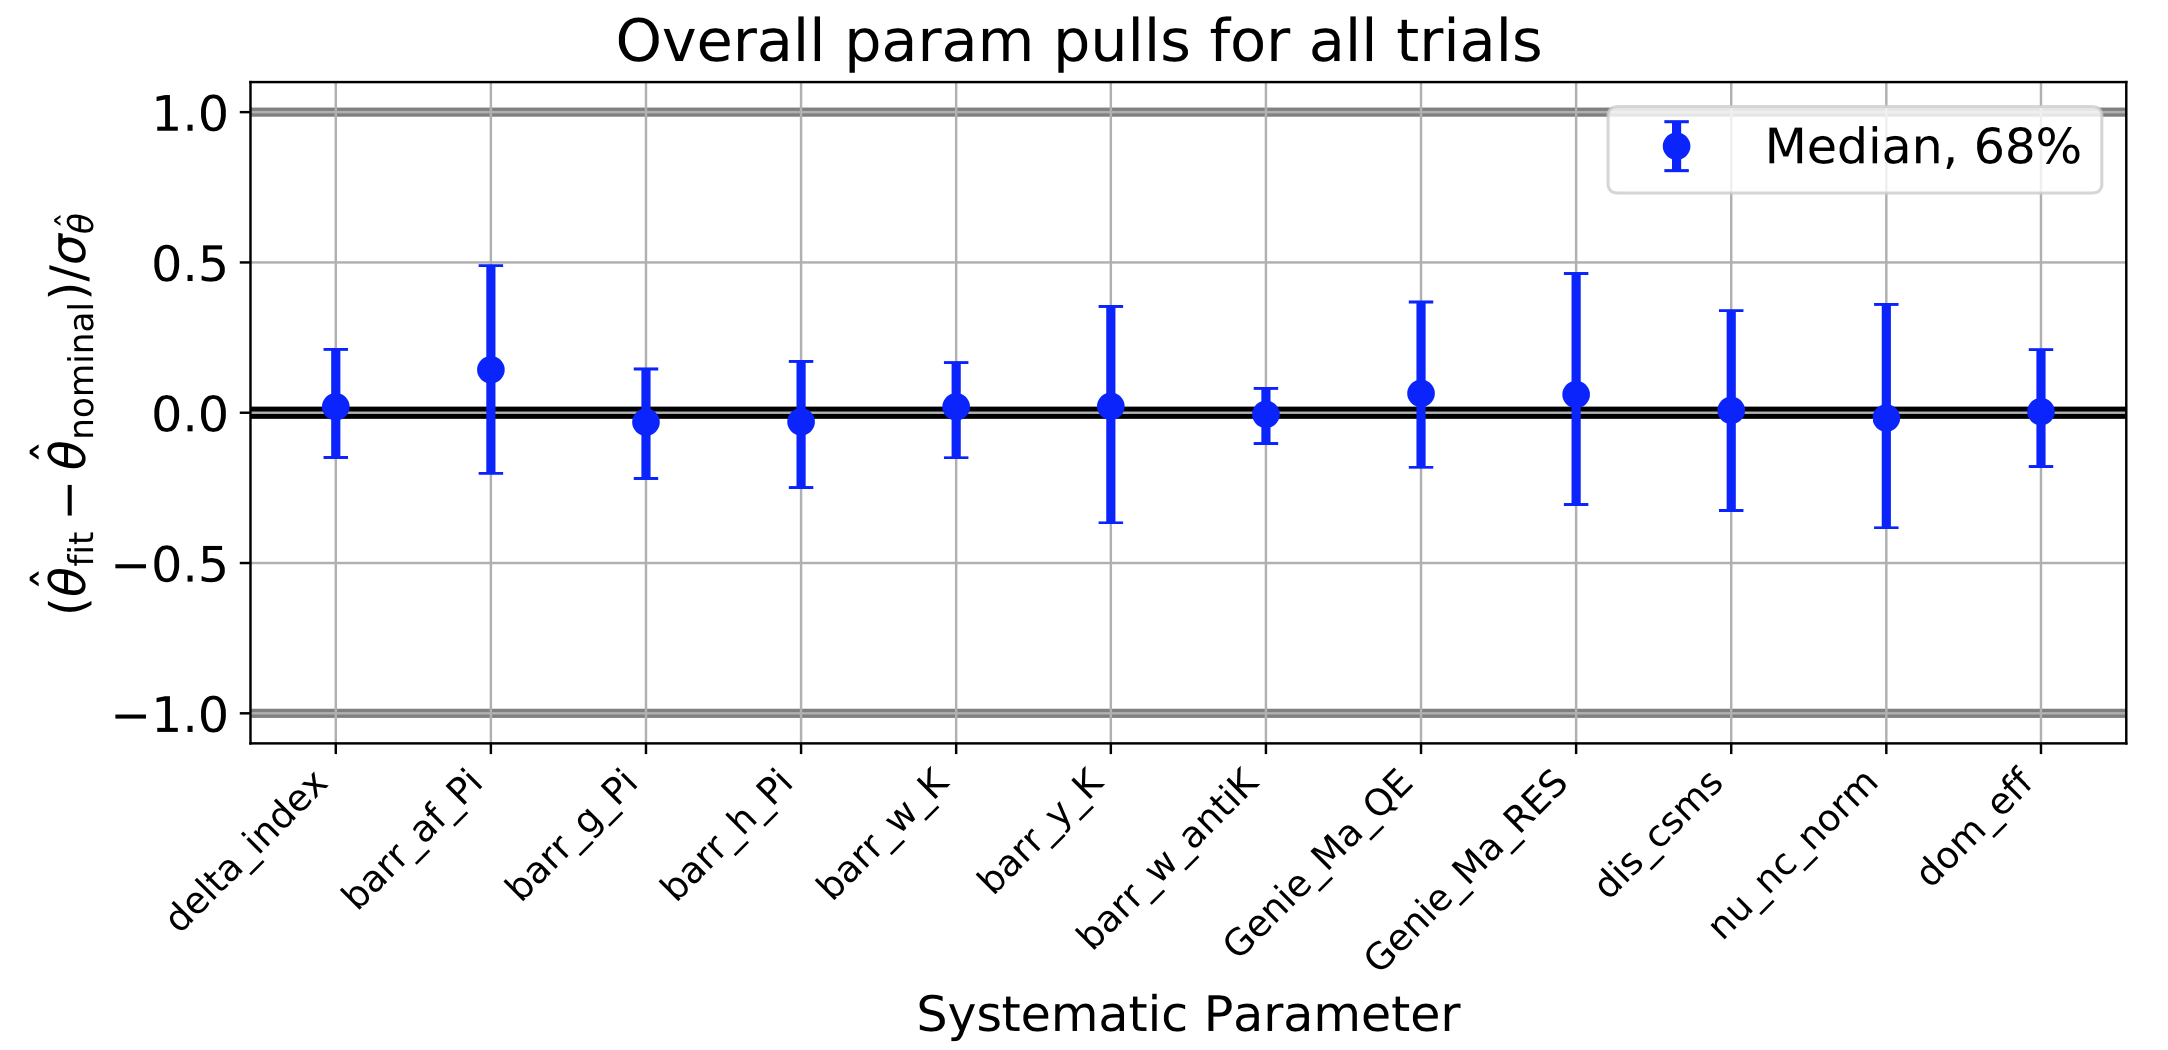
\includegraphics[width=0.99\textwidth]{figures/measurement/three_flavor/ensemble_pre_fit/ensemble_pull.png}  
    \end{subfigure}
  \caption{Distributions of fitted values of each parameter considered in the three-flavor analysis (top), and their corresponding pulls from nominal (bottom).
  \label{fig:three-flavor-ensemble-param}}
\end{figure}

\subsection{Results}

\subsubsection{Goodness of Fit}

Before looking at the best fit parameters of the real data fit, the goodness of fit is assessed using the total and bin-wise test statistic distributions. The distribution of the test statistic acquired from the ensemble described in \refsec{three-flavor-ensemble} is shown in \reffig{three-flavor-ts-ensemble} together with the observed test statistic from real data. The observed test statistic is found to lie very well within the expectation with a p-value of 32\%. The bin-wise contribution and the test statistic and its expected distribution are shown in \reffig{three-flavor-binwise-ts}. The histogram shows no apparent regions of particularly bad agreement between data and the the MC expectation, and the distribution of the bin-wise test statistic is in agreement with the distribution expected from pseudo-data trials.

\begin{figure}
    \centering
    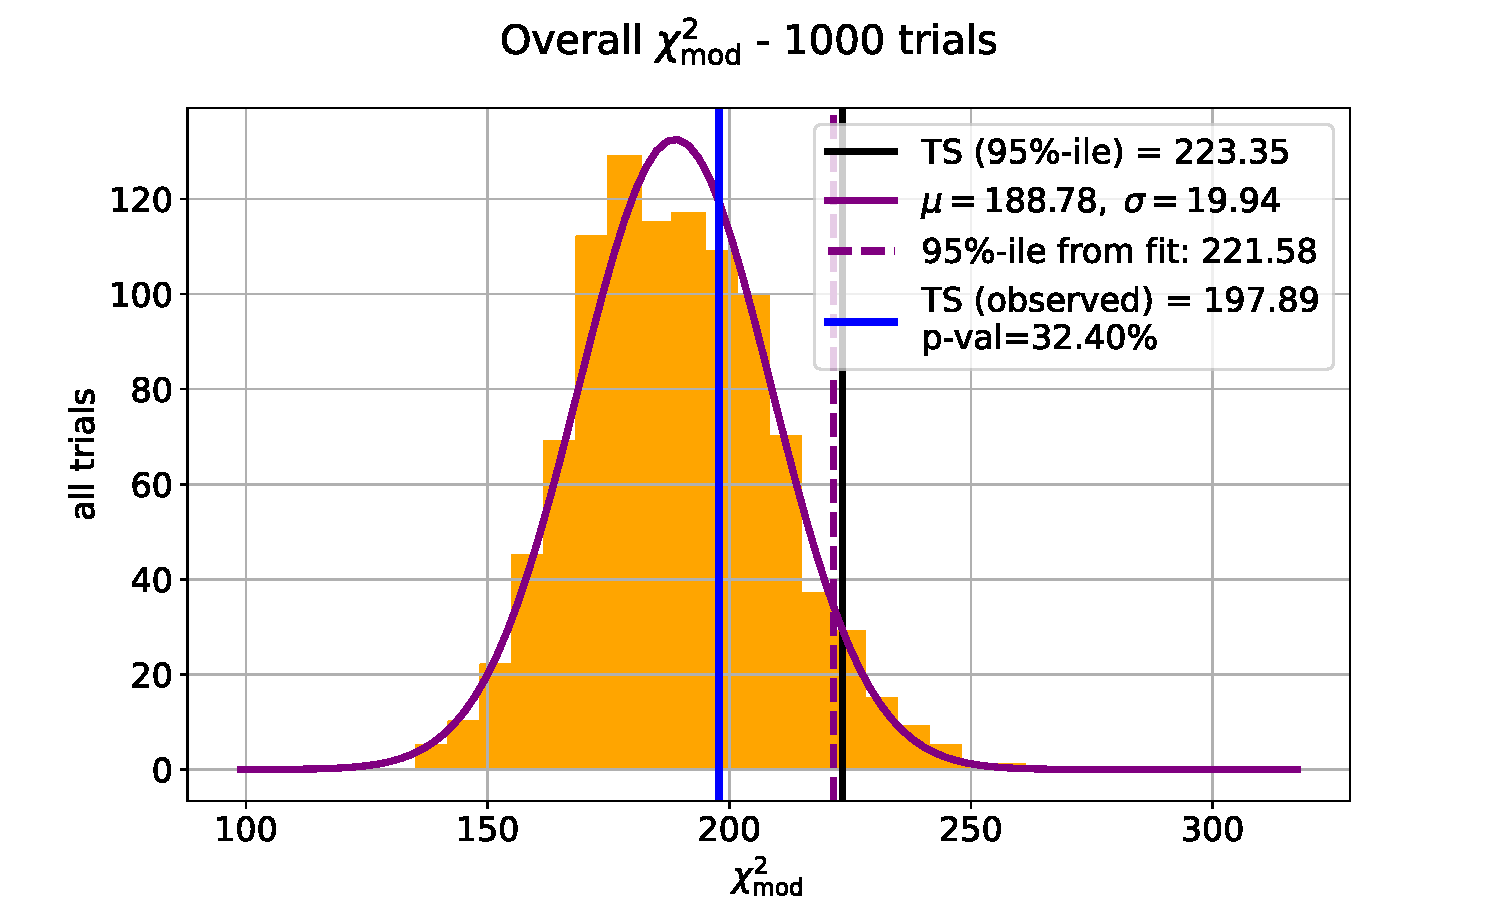
\includegraphics[width=0.8\linewidth]{figures/measurement/three_flavor/ensemble_pre_fit/overall_ts_wings_trials.pdf}
    \caption{Observed test statistic value of the three-flavor oscillation analysis compared to expected distribution from ensemble.}
    \label{fig:three-flavor-ts-ensemble}
\end{figure}

\begin{figure*}
    \centering
    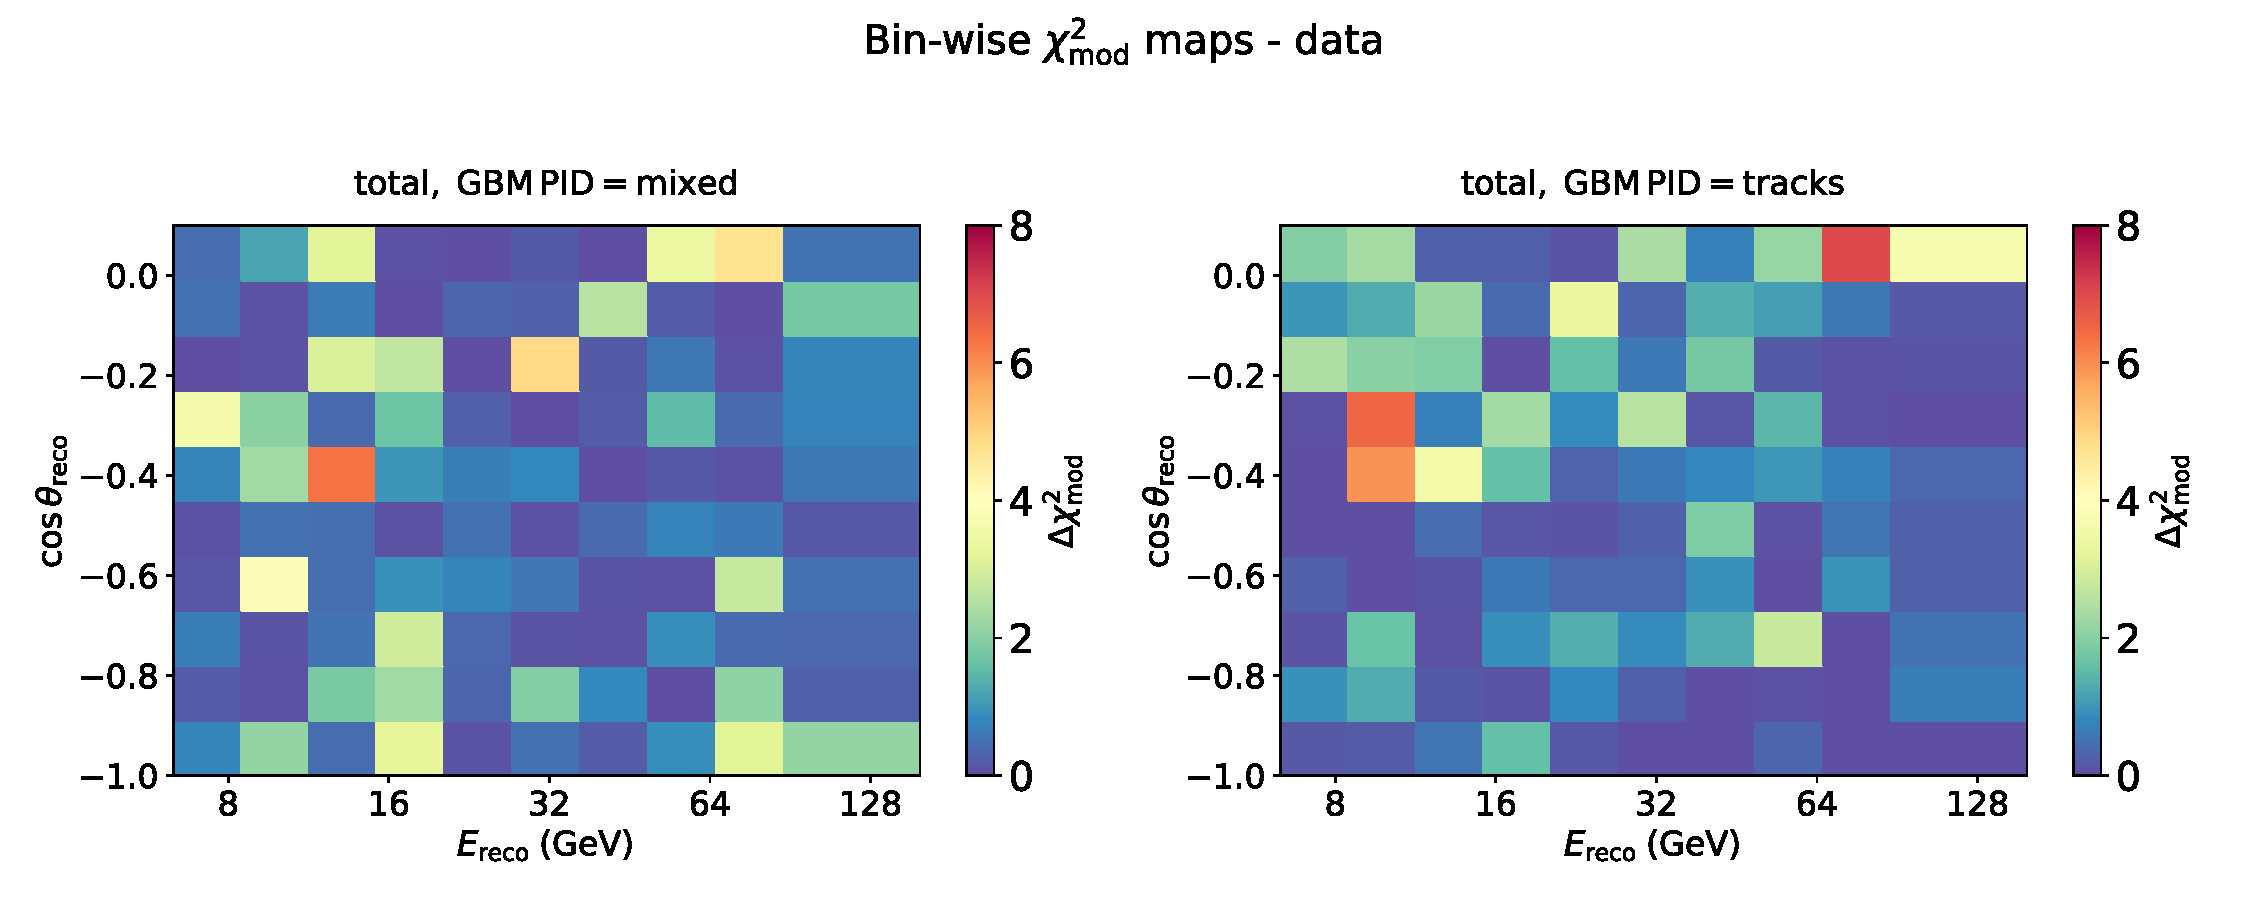
\includegraphics[height=0.22\linewidth]{figures/measurement/three_flavor/ensemble_pre_fit/real_fit_binwise_pulls_pre_bugfix.pdf}
    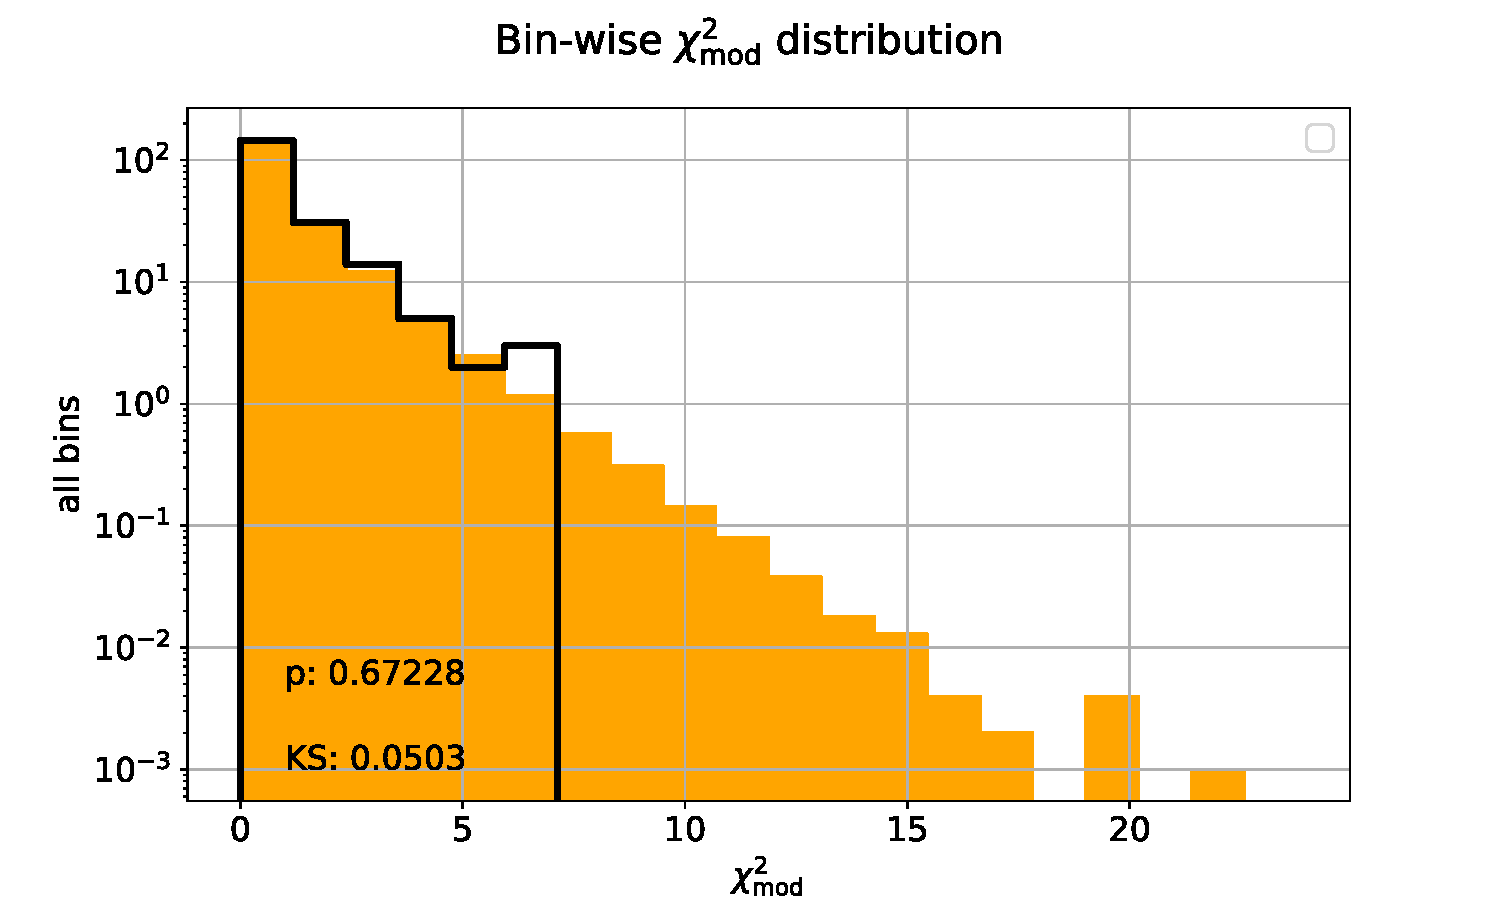
\includegraphics[height=0.22\linewidth]{figures/measurement/three_flavor/ensemble_pre_fit/binwise_ts_wings_trials.pdf}
    \caption{Contribution of every bin to the over-all test statistic in the three-flavor analysis (left) and their observed distribution compared to the expected distribution from pseudo-data trials (right).}
    \label{fig:three-flavor-binwise-ts}
\end{figure*}

\subsubsection{Test for un-physical mixing}
If the real data contains an under-fluctuation in the oscillation valley, it is possible that the fit prefers more than maximal $\nu_\mu$ disappearance, which is physically not possible. This tendency to fit un-physical magnitudes of $\nu_\mu$ disappearance is tested by running a fit in which the oscillation probabilities are calculated with a simplified two-flavor equation in which the scale of the oscillation, $\sin^2(2\theta_{23})$\todo{explain this simplification in the theory section and link here}, is replaced with a scaling factor that is allowed to float freely even to un-physical values where $\sin^2(2\theta_{23}) > 1$. If the true mixing angle is $\theta_{23}=45^\circ$, it is expected that such un-physical best-fit values can occur solely due to random Poisson fluctuations of the data. To quantify this expectation, another ensemble of trials is produced in the way described in \refsec{three-flavor-ensemble}, where the injected true mixing is maximal. The two flavor analysis is run on each trial to produce a distribution of expected values that is shown in \reffig{two-flavor-ensemble}\todo{draw the observed value in the figure}. The results show that, while the real data fit does indeed prefer a slightly un-physical $\nu_\mu$ disappearance, this preference still lies well within the expectation if the true mixing was assumed to be maximal.

\begin{figure}
    \centering
    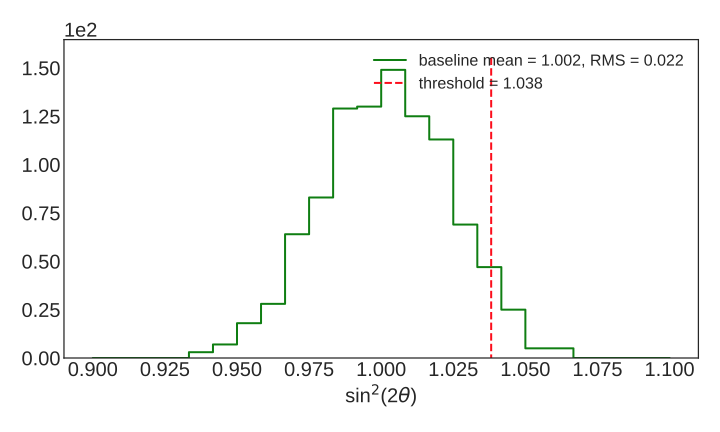
\includegraphics[width=0.8\linewidth]{figures/measurement/three_flavor/ensemble_pre_fit/two_flav_ensemble_threshold.png}
    \caption{Observed best fit values of the two-flavor fit compared to the distribution from pseudo-data trials.}
    \label{fig:two-flavor-ensemble}
\end{figure}

\subsubsection{Measured Nuisance Parameter Values}
After first having established that the goodness of fit variables and the magnitude of the un-physical disappearance lie within the expectation from pseudo-data trials, the best-fit values of the nuisance parameters are revealed. The results are shown in \reftab{nuisance_params_fittedval}. The pull values show that all parameters fit comfortably within $1\sigma$ of their defined priors. The fit prefers a slightly harder cosmic ray spectrum and a larger muon background than initially expected. The optical efficiency of the DOMs fits to a slightly larger value than nominal with 106\%, while the ice properties stay very close to their initial values.

%The hole ice parameters prefer less acceptance of photons entering the DOMs directly from below, and the shape of their corresponding acceptance curve is close to the best fit result from LED flasher studies\todo{cite hole ice flasher studies} as shown in \reffig{hole-ice-flasher-comparison-three-flavor}.

\begin{table}
    \centering
    \caption{Fitted values of all nuisance parameters from the all-season three-flavor fit. The pull of the best fit value is shown for parameters with a defined prior.}
    \label{tab:nuisance_params_fittedval}
    \begin{tabular}{lSS} \toprule
        Parameter  & {Best Fit Value} &  {Pull ($\sigma$)} \\ \midrule
        delta index & 0.065 & 0.648 \\
        barr af Pi & 0.221  & 0.351 \\
        barr g Pi & -0.053  & -0.175 \\
        barr h Pi & -0.016  & -0.11 \\
        barr w K & 0.079  & 0.198 \\
        barr y K & 0.102  & 0.341 \\
        barr w antiK & -0.010  & -0.0244 \\
        $M_{A}^{CCQE}$ &  0.043 & 0.043 \\
        $M_{A}^{CCRES}$ & 0.607 & 0.607  \\
        dis csms & 0.027  & 0.0267 \\ 
        $A_{eff}$ scale & 0.823 &  \\
        NC normlisation & 1.121 &  0.605 \\
        DOM efficiency & 1.065  & 0.647 \\
        hole ice p0 & -0.267  &  \\
        hole ice p1 & -0.042  &  \\
        ice absorption & 0.973  &  \\
        ice scattering & 0.988 &  \\ 
        Weight scale & 1.371  &  \\
        \bottomrule
    \end{tabular}
\end{table}

% \begin{figure}
%     \centering
%     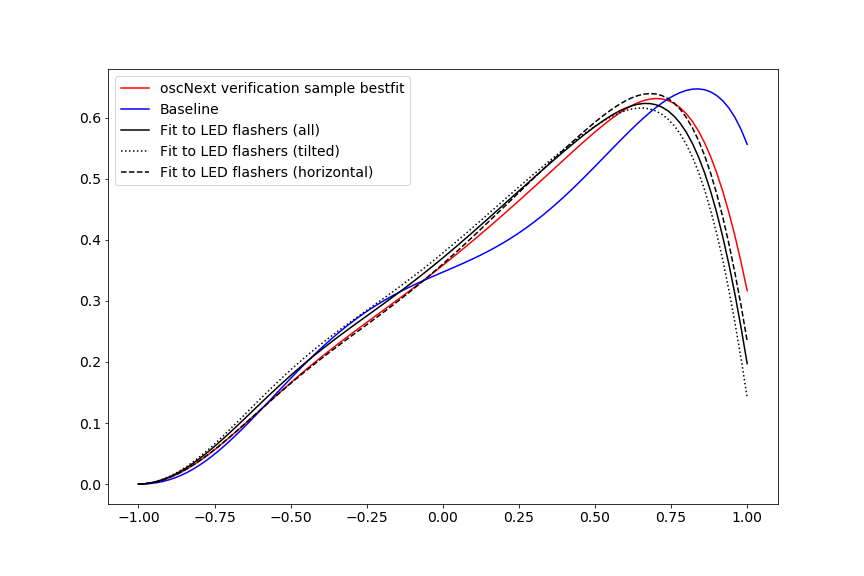
\includegraphics[width=0.8\linewidth]{figures/measurement/three_flavor/results/hole_ice_curve_best_fit.png}
%     \caption{Acceptance curve corresponding to the best-fit hole ice parameters of the three-flavor analysis compared to the baselind and the results of IceCube flasher studies.}
%     \label{fig:hole-ice-flasher-comparison-three-flavor}
% \end{figure}

\subsubsection{Oscillation parameters}
The fitted values for the three-flavor oscillation parameters are $\theta_{23} = 45.3639$ and $\Delta m^2_{31} = 2.47996 \times10^{-3}$ eV$^2$, which corresponds to $\sin^2\theta_{23} = 0.505$ and $\Delta m^2_{32} = 2.41 \times10^{-3}$ eV$^2$. The 90\% C.L. allowed region for these parameters is shown in \reffig{real_data_contour_three_flavor} compared to measurements from other experiments. The observed 90\% range for $\theta_{23}$ is [40.866, 49.685] and is slightly smaller than the expected Asimov contour at the best fit point. To make sure that this is compatible with random fluctuations, the likelihood is profiled over $\sin^2(\theta_{23})$ for 1000 pseudo-data trials. \reffig{mixing_brazil_band_three_flavor} shows the  68\% (90\%) intervals of the test statistic at each point of the scan over all trials. The observed contour is fully contained in the 68\% band, demonstrating that the narrowed 90\% range for $\theta_{23}$ is fully compatible with expected data fluctuations.

\begin{figure}
    \centering
        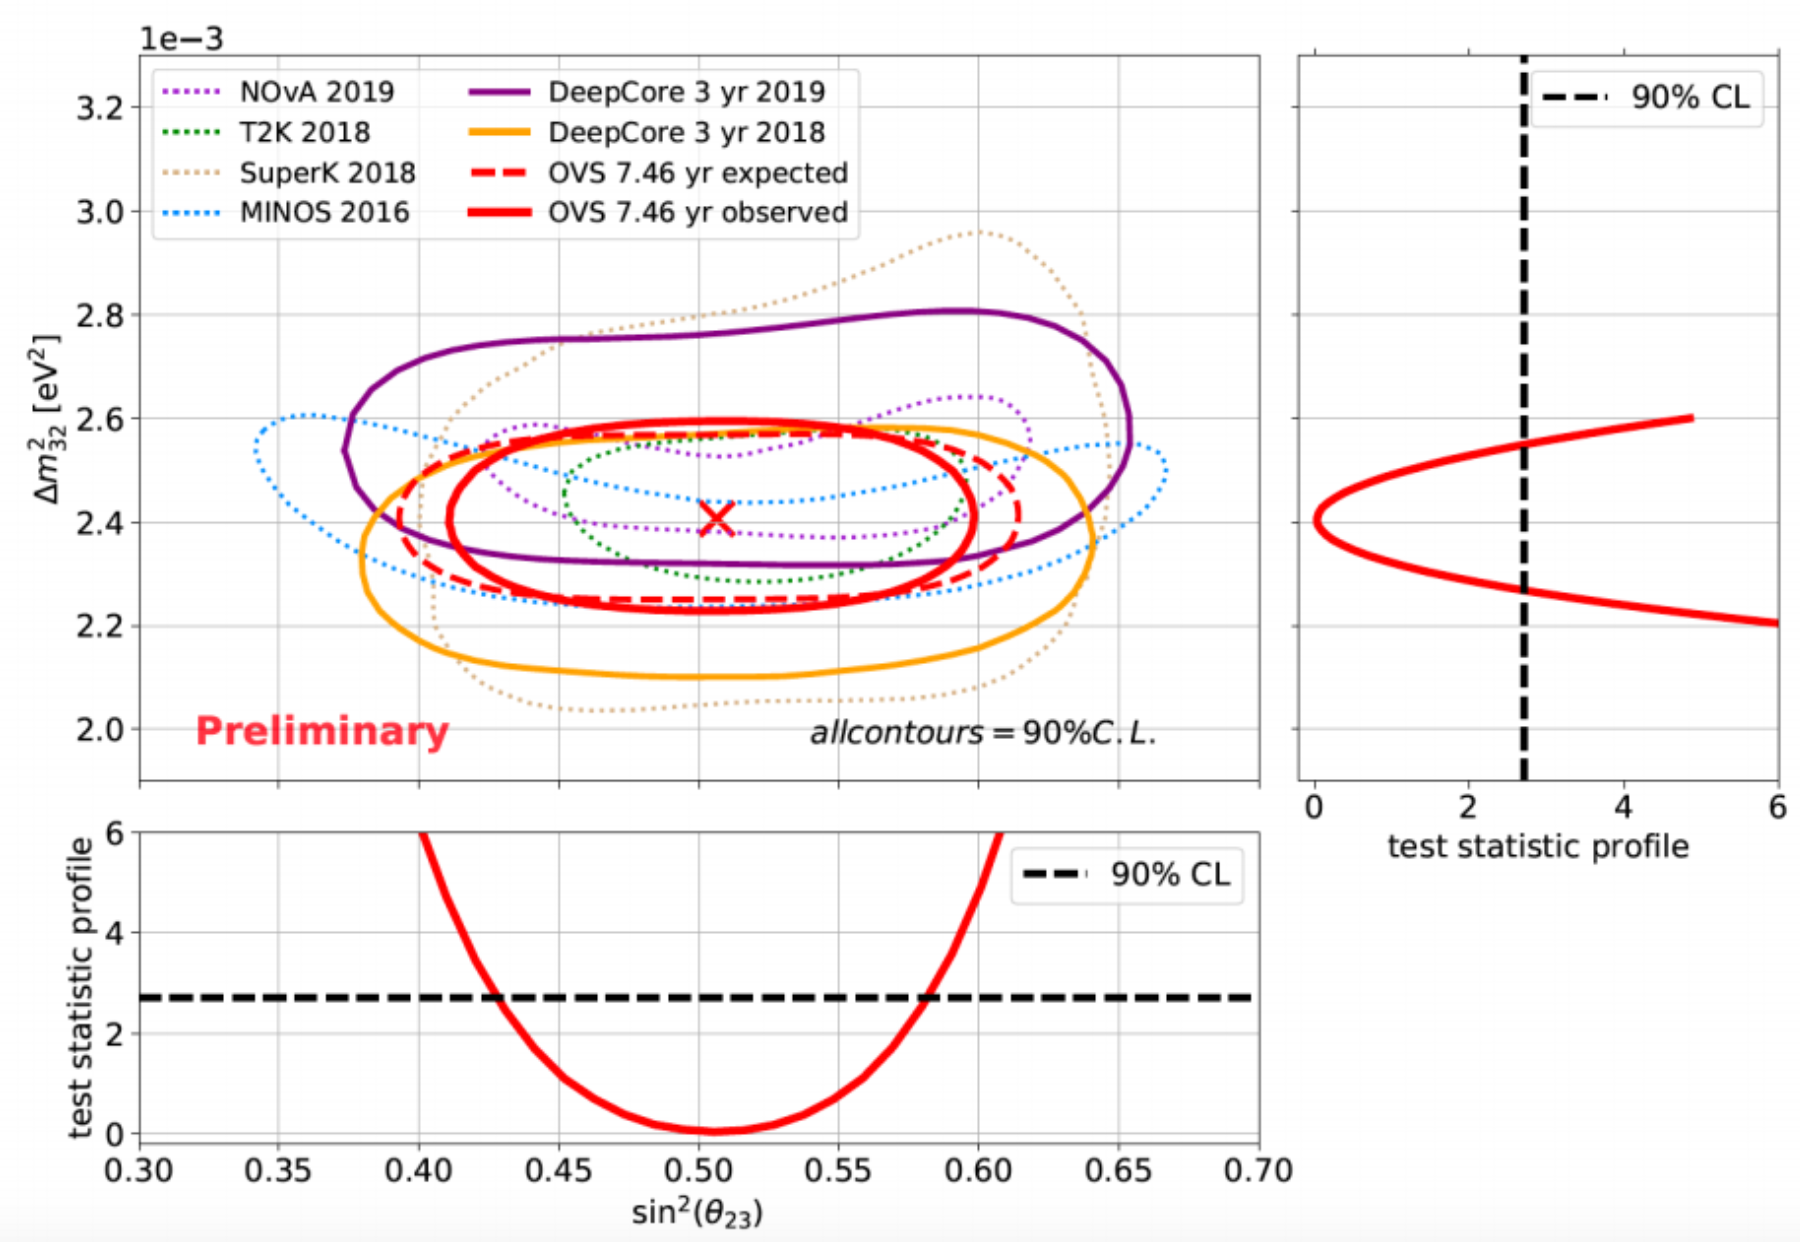
\includegraphics[width=0.9\textwidth]{figures/measurement/three_flavor/results/real_data_contour.png}  
  \caption{Contours showing the 90\% C.L. allowed region for the physics parameters of the three-flavor analysis. The red solid(dash) contours represent the observed(expected) sensitivity. The cross shows the best fit value. The bottom and right plots show the 1D likelihood profiles for $sin^2\theta_{23}$ and $\Delta m^2_{32}$, respectively. 
  \label{fig:real_data_contour_three_flavor}}
\end{figure}

\begin{figure}
    \centering
        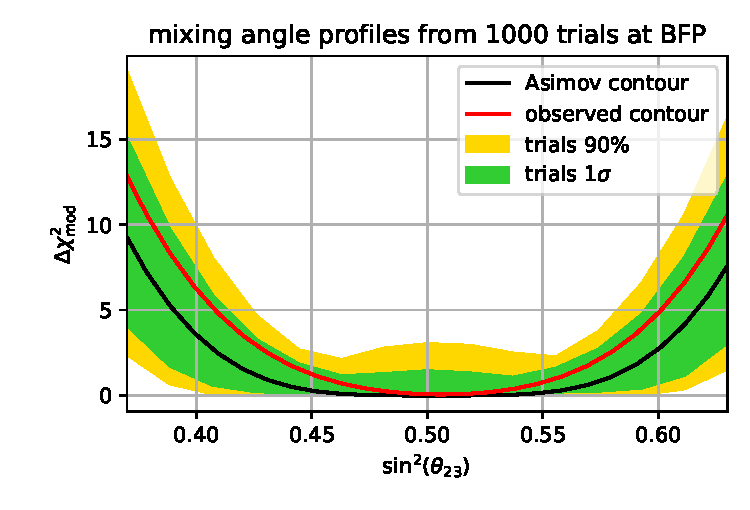
\includegraphics[width=0.8\textwidth]{figures/measurement/three_flavor/results/mixing_brazil_band.pdf}  
  \caption{Observed contour in $\sin^2(\theta_{23})$ (red) compared to the Asimov expectation (black) and the distribution of 1000 pseudo-data trials (yellow and green bands) produced at the best fit point of the three-flavor oscillation analysis. The observed contour is fully contained within 68\% of the fluctuations of the trials.
  \label{fig:mixing_brazil_band_three_flavor}}
\end{figure}

\subsubsection{Likelihood Coverage}

When drawing the 90\% exclusion contour shown in \reffig{real_data_contour_three_flavor}, it is assumed that Wilks' theorem holds, that is, the distribution of the test statistic follows a $\chi^2$ distribution with two degrees of freedom. If this assumption holds, then the value of the test statistic should lie below the 90\% threshold for 90\% of repeated independent measurements. The relationship between the expected percentiles and the true distribution is referred to as \emph{coverage}. If more than 90\% of repeated measurements fall below the 90\% threshold, the likelihood is said to be \emph{over-covering}. In the reverse case where fewer than 90\% of repeated measurements fall below the 90\% threshold, the likelihood is said to be \emph{under-covering}. The coverage of the likelihood may change depending on the assumed true parameter values. For this measurement in particular, it is expected that the likelihood should over-cover near maximal mixing, because the mixing angle can no longer provide a full degree of freedom. To test the coverage for particular values of $\theta_{23}$ and $\Delta m^2_{31}$, pseudo-data is generated where these values are injected as true values. The bin counts of the pseudo-data are Poisson-fluctuated to create an ensemble of trials. Then, one free fit is run, and another fit where the physics parameters are fixed to their true values. The coverage is then evaluated by counting the fraction of trials for which $\Delta \chi^2_{\mathrm{mod}}$ between these two fits is smaller than the 90\% threshold given by Wilks' theorem. The results are shown in \reffig{three-flavor-coverage} for a range of points in mixing angle and mass splitting. As expected, the likelihood is over-covering near maximal mixing, while there is very little dependence of the coverage on the mass splitting. The likelihood is over-covering for all points in mass splitting in the right panel of \reffig{three-flavor-coverage}, because the injected mixing angle was at the best fit point of the analysis, which is very close to maximal. In conclusion, the 90\% contours shown in \reffig{real_data_contour_three_flavor} are slightly over-conservative in the region close to maximal mixing.

\begin{figure*}
    \centering
    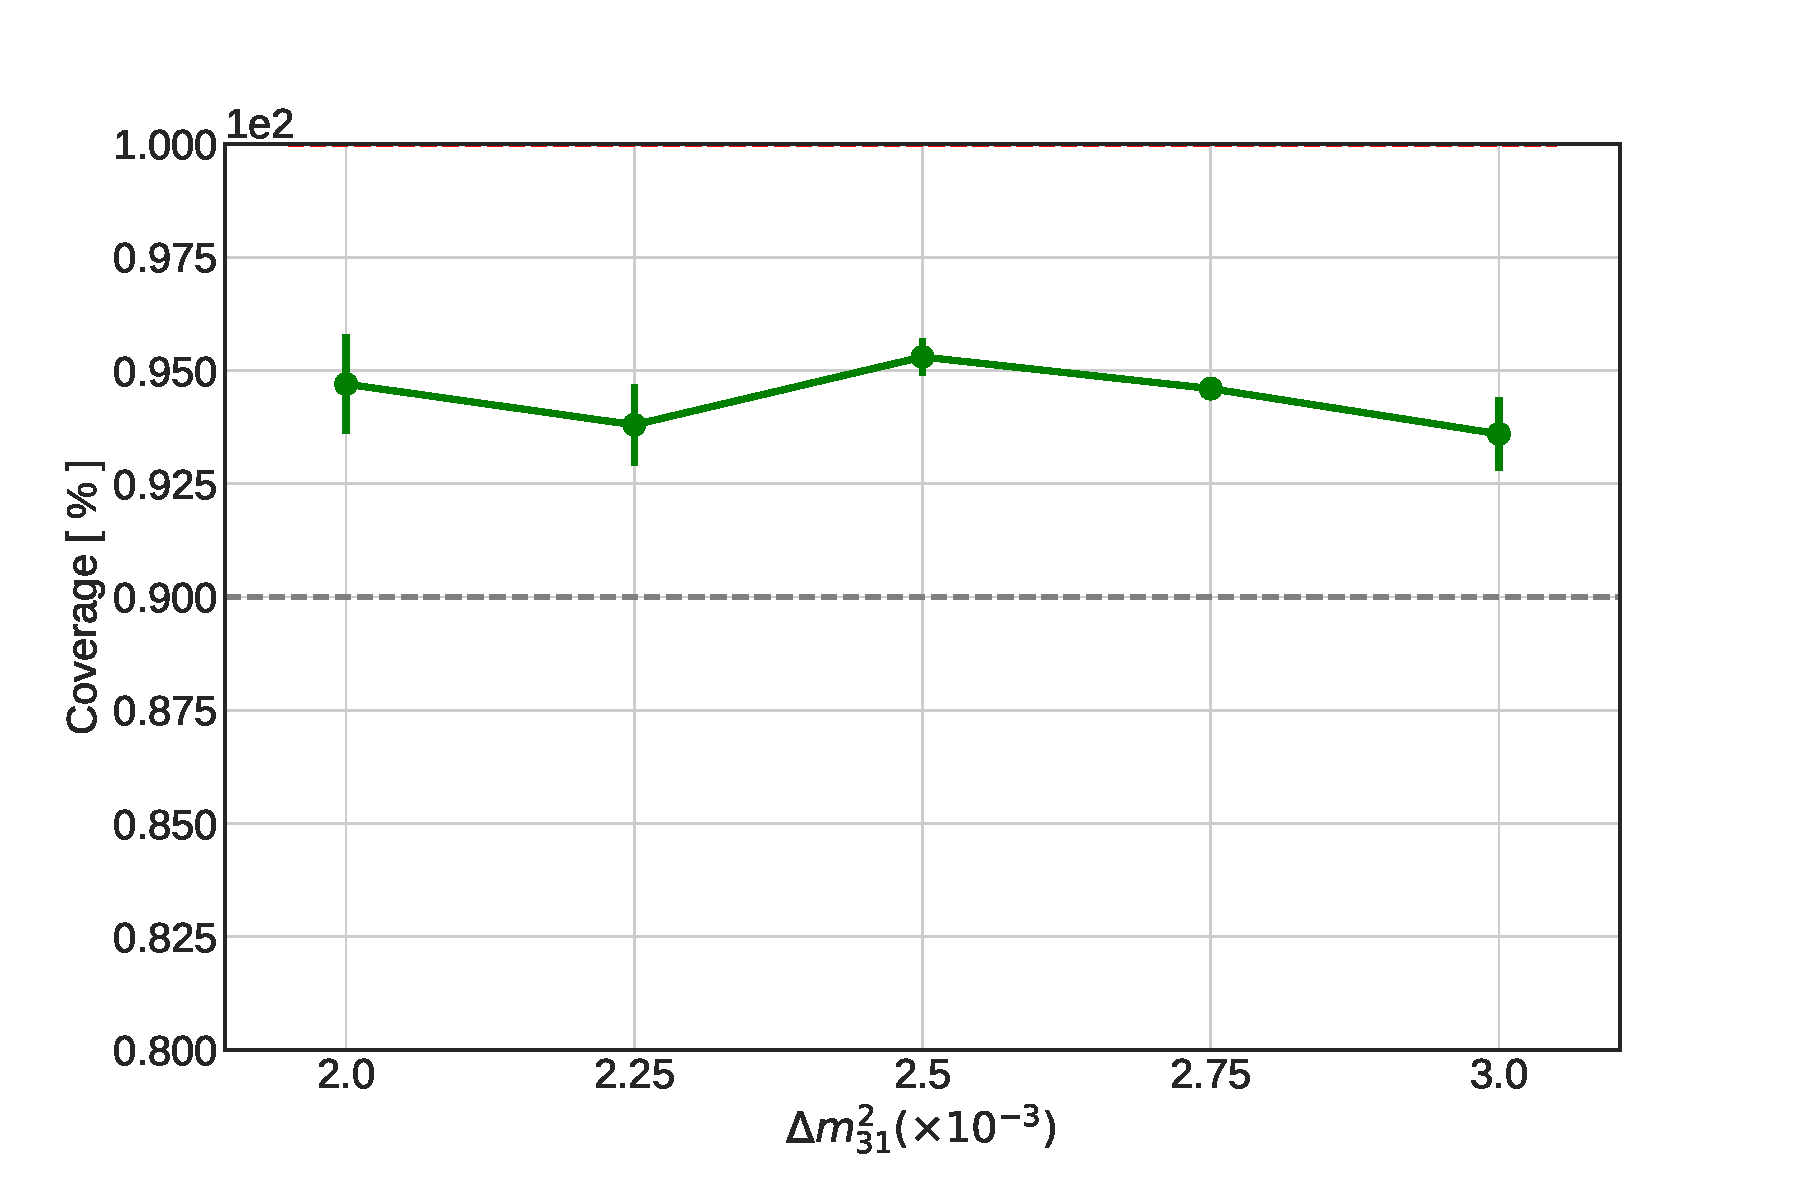
\includegraphics[width=0.45\linewidth]{figures/measurement/three_flavor/coverage_test/coverage_dm_v3.pdf}
    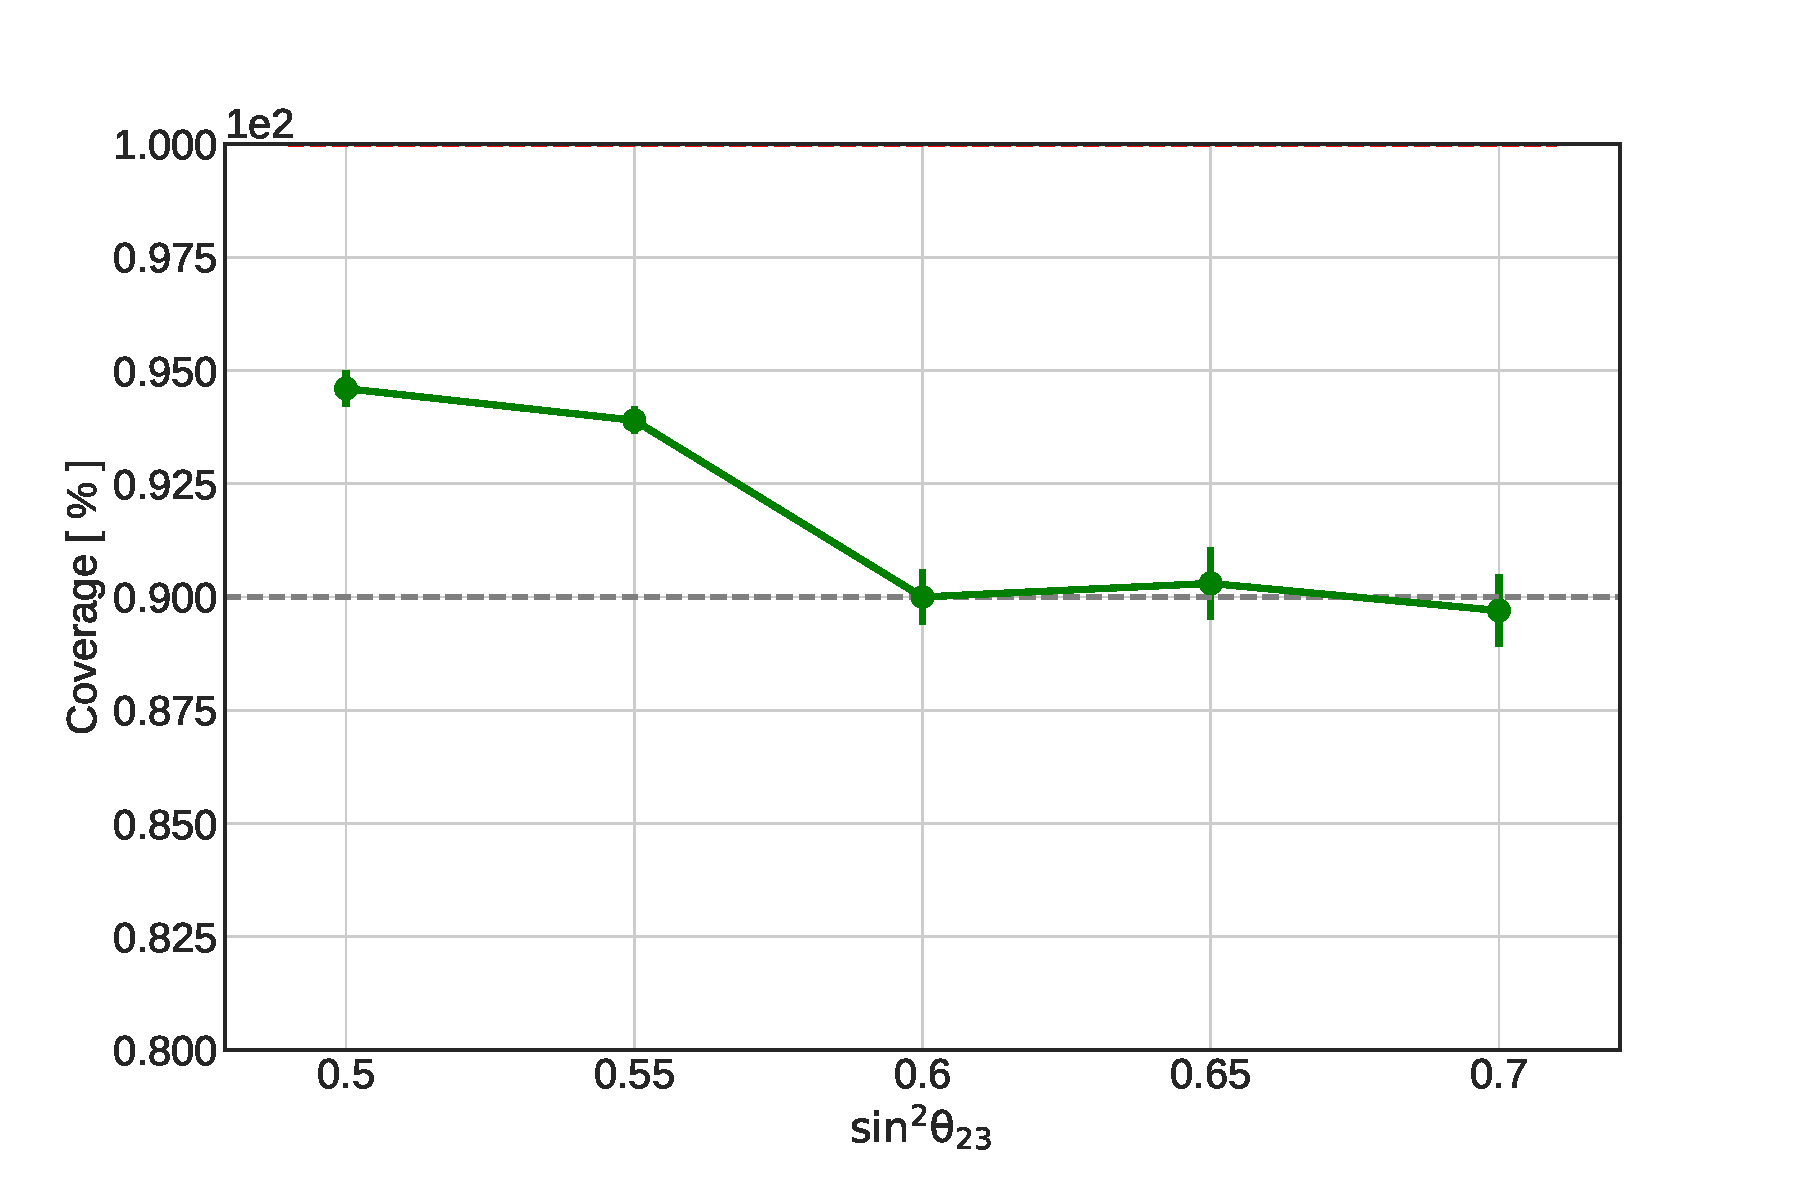
\includegraphics[width=0.45\linewidth]{figures/measurement/three_flavor/coverage_test/coverage_t23_v3.pdf}
    \caption{Fraction of trials below the 90\% threshold expected from Wilks' theorem for a range of points in mass splitting (left) and mixing angle (right).}
    \label{fig:three-flavor-coverage}
\end{figure*}